\documentclass{article}

\usepackage{graphicx}
\usepackage{tikz}
\usepackage{tikzsymbols}
\usetikzlibrary{calc,patterns,shapes.geometric}
\pagestyle{empty}
\usepackage[margin=0pt]{geometry}
\geometry{papersize={14in,12in}}

\def\centerarc[#1](#2)(#3:#4:#5){\draw[#1] ($(#2)+({#5*cos(#3)},{#5*sin(#3)})$) arc (#3:#4:#5);}

\begin{document}
	\begin{figure}
		\centering
		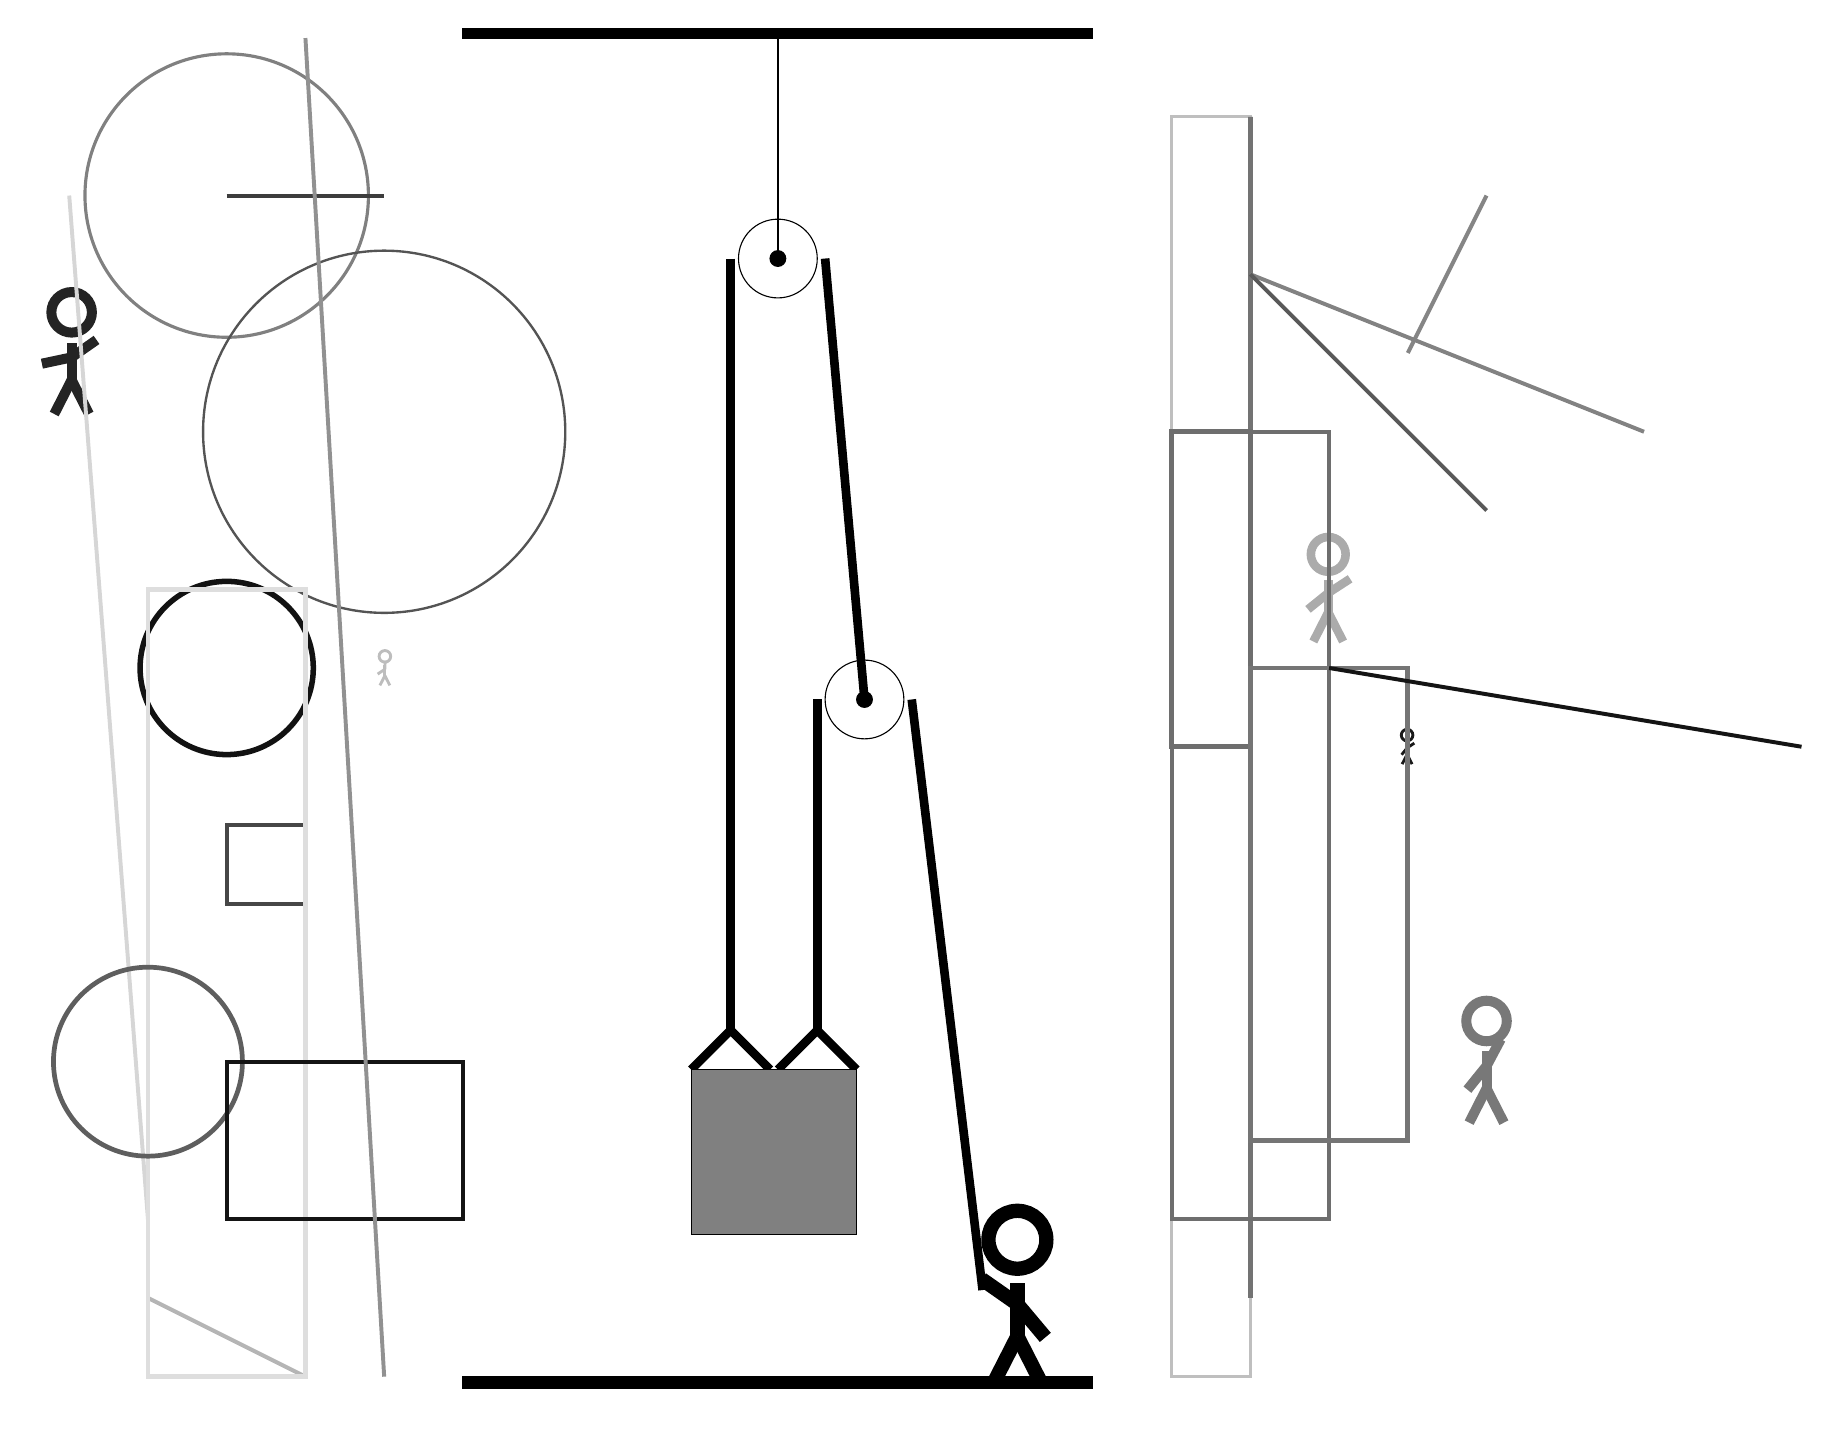
\begin{tikzpicture}
			%%%%% START %%%%%
			
			\draw[fill=black] (-2, 14) rectangle (6, 14.125);
			
			\draw[line width=0.5mm, color=black!72] (-4, 4) rectangle (-5, 3);
			
			\draw[line width=0.5mm, color=black!29](-6, -2) -- (-4, -3);
			\draw [line width=0.4mm, color=black!50](-5, 12) circle (1.8);
			\node[line width=0.3mm, color=black!26] at (-3, 6) {\Strichmaxerl[2][34][88]};
			\draw[line width=0.4mm, color=black!25] (8, 13) rectangle (7, -3);
			\draw[line width=0.5mm, color=black!48](10, 10) -- (11, 12);
			\node[line width=0.3mm, color=black!86] at (-7, 10) {\Strichmaxerl[7][12][35]};
			\draw[line width=0.2mm, color=black!35] (-4, 6) rectangle (-4, 5);
			\draw [line width=0.3mm, color=black!67](-3, 9) circle (2.3);
			\node[line width=0.2mm, color=black!33] at (9, 7) {\Strichmaxerl[6][39][33]};
			
			\draw[line width=0.7mm, color=black!55] (8, -2) rectangle (8, 13);
			
			\draw[line width=0.5mm, color=black!76](-5, 12) -- (-3, 12);
			\draw[line width=0.5mm, color=black!16](-6, -1) -- (-7, 12);
			
			\draw [line width=0.7mm, color=black!93](-5, 6) circle (1.1);
			\draw[line width=0.5mm, color=black!49](8, 11) -- (13, 9);
			\draw[line width=0.6mm, color=black!13] (-4, 7) rectangle (-6, -3);
			\draw [line width=0.6mm, color=black!63](-6, 1) circle (1.2);
			
			\draw[line width=0.5mm, color=black!92] (-2, -1) rectangle (-5, 1);
			\node[line width=0.5mm, color=black!90] at (10, 5) {\Strichmaxerl[2][51][34]};
			
			\draw[line width=0.6mm, color=black!57] (7, 9) rectangle (8, 5);
			\draw[line width=0.5mm, color=black!57] (7, -1) rectangle (9, 9);
			\draw[line width=0.6mm, color=black!54] (8, 0) rectangle (10, 6);
			\draw[line width=0.5mm, color=black!92](9, 6) -- (15, 5);
			\draw[line width=0.5mm, color=black!43](-3, -3) -- (-4, 14);
			\node[line width=0.6mm, color=black!53] at (11, 1) {\Strichmaxerl[7][51][62]};
			
			\draw[line width=0.5mm, color=black!65](8, 11) -- (11, 8);
			
			
			\draw (2, 11.2) circle (0.5);
			\draw[fill=black] (2, 11.2) circle (0.1);
			\draw[thick] (2, 11.2) -- (2, 14);
			
			\draw (3.1, 5.6) circle (0.5);
			\draw[fill=black] (3.1, 5.6) circle (0.1);
			
			\draw[line width = 1.1mm]  (0.9, 0.9) -- (1.4, 1.4) -- (1.9, 0.9);
			\draw[line width = 1.1mm]  (2.0, 0.9) -- (2.5, 1.4) -- (3.0, 0.9);
			\draw[fill=black!50] (0.9, 0.9) rectangle (3.0, -1.2);
			
			\draw[line width = 1.1mm] (1.4, 11.2) -- (1.4, 1.4);
			\centerarc[line width = 1.1mm](2, 11.2)(0:180:0.6);
			\draw[line width = 1.1mm] (2.6, 11.2) -- (3.1, 5.6);
			\draw[line width = 1.1mm] (2.5, 5.6) -- (2.5, 1.4);
			\centerarc[line width = 1.1mm](3.1, 5.6)(0:180:0.6);
			\draw[line width = 1.1mm] (3.7, 5.6) -- (4.6, -1.9);
			
			\node at (5, -2) {\Strichmaxerl[10][-35][-50]};
			
			\draw[fill=black] (-2, -3) rectangle (6, -3.15);
			
			%%%%% END %%%%%
		\end{tikzpicture}
	\end{figure}	
\end{document}